\documentclass[a4paper, 11pt]{article}

\usepackage{graphicx}

\author{Yang Zheng (5120379052)\\\small{@SE, SJTU}}
\title{Data Structure Project\\\large{Social Network}}
\date{}
\begin{document}
\maketitle
\tableofcontents
\section{Abstract}
This document introduces some details about my data structure project, which finished a simple social network program using B-tree and list.

\section{Functions \& Interfaces}
\subsection{Sign in \& Sign up}
Input your account and password to sign in. Start account with `!' to sign up.

The corresponding member functions in class `User' are `set' and `newAccount'. For storage in background, methods `get' and `newAccount' belonging to class `UserInfo' are responsible.

\subsection{Change \& get profile}
After loging in, you can input `info' to show your profile and input `pw', `addrss', `birth', `tele' or `gender' to modify them.

The corresponding member functions in class `User' are `password', `addree', `birthday', `telephone' and `gender'. The method in `UserInfo' is `alter'.

\subsection{Circle}
You can input `follow' to follow someone or `unfollow' to unfollow. Entering `follower' or `following' will display your followers and following list.

The names of interfaces are the same as above.

\subsection{Message}
To publish a message, you can input `message'. Entering `list' will display your and your followings' recent messages. Also, you can give `visit' to list specific user's messages.

The interface to messaging is `message' in `User' and `list' is responsible for `list' and `visit' functions. The names in background class are the same as foreground.

\subsection{Close account}
Input `close' to close your account and no one could register this name anymore.

The corresponding methods are `close' in `User' and `remove' in `UserInfo'.

\section{Implementation}
\subsection{User information}
The detail profile data of users is in `user.dat'. The number of users is indicated by `index.dat' and the structure is B-tree stored in `snapshot.dat'. This B-tree is indexed by string(array of char) and stores the IDs related to the offset in the file of users.

\subsection{Relationship}
The following relation is stored in `follower.dat' and `following.dat' using B-trees too. These trees are organized by the IDs of users. Every user has spaces for the respective positions of roots in two files.

\subsection{Messages}
The messages are stored in `message.dat' by the order of time. For every user's messages, it uses list to solve it. Every time a user asked for a message list, it reads every message one by one and check if the publisher is one of his or her following user.

\subsection{B Tree}
The B-tree is implemented in `btree.hpp' using template. You can change the degree `D' and every tree is related to a specific file and a offset to root. Keys and values of the tree are arrays of scalars.

\section{Efficiency}
This project implemented a version origanizes user's profiles using brute force and a version using B-tree. So the comparison of these two are givin. Also, it gave the test results of situations with different B-tree degrees.

The test program is `test.cpp' in the folder `client' and you can type `make test' in terminal to compile test program.

All of the following figures are based on datas from `documentation/raw'.

\begin{flushleft}
  Environment:
  \begin{small}
    \begin{description}
    \item[System:] ArchLinux, Linux Kernel 3.13.5-1-ARCH
    \item[CPU:] Intel(R) Core(TM) i3-2330M CPU @ 2.20GHz, 2 cores, 2 threads per core
    \end{description}
  \end{small}
\end{flushleft}

\subsection{Comparison between brute-force and B-tree}
To compare the efficiency differences of brute-force algorithm and B-tree implementation, it tests from 10 to 100000 operations.

Figure \ref{bruteVSbtree10} are the plots for 10\% operations being creating an account.
\begin{figure}[htbp]
  \centering
  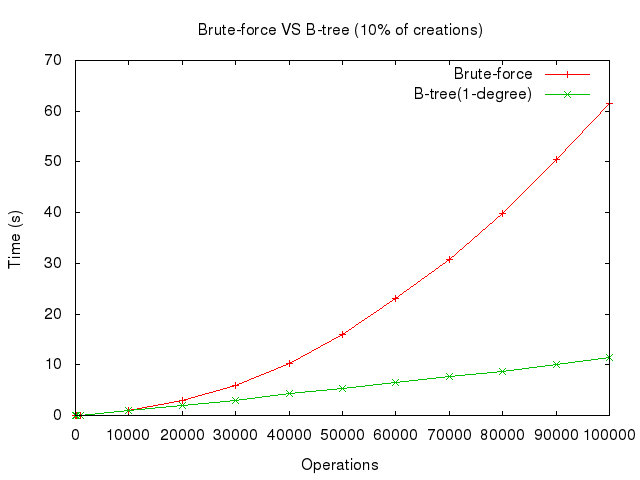
\includegraphics[width=0.95\textwidth]{./plots/bruteVSbtree10.png}
  \caption{Brute-force VS B-Tree (10\% of insertions)}
  \label{bruteVSbtree10}
\end{figure}

Figure \ref{bruteVSbtree30} are the plots for 30\% operations opertions being creating an account.
\begin{figure}[htbp]
  \centering
  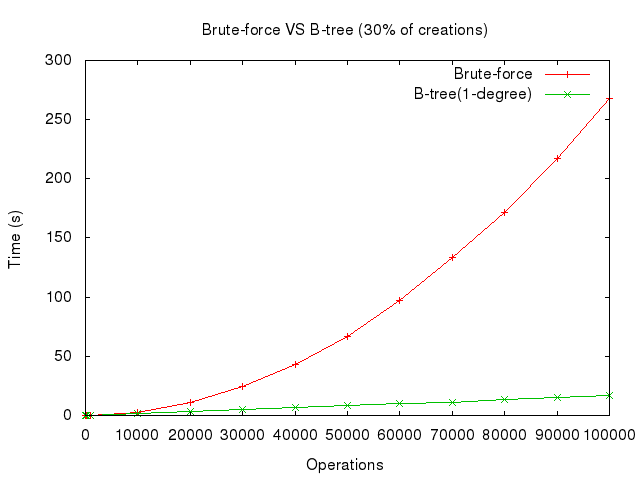
\includegraphics[width=0.95\textwidth]{./plots/bruteVSbtree30.png}
  \caption{Brute-force VS B-Tree (30\% of insertions)}
  \label{bruteVSbtree30}
\end{figure}

From above plots, we can figure out that, brute-force algorithm may be the complexity of $O(N^2)$ and the B-tree implementation can be nearly seemed as $O(N)$ although it's $O(N\log{N})$ in fact.

\subsection{Comparison among different degrees}
It tested degrees of B trees from 1 to 30, operations varied from 10 to operations and the proporions varied from 10\% to 70\%.

Figure \ref{cmpLOT10} are the plots for 10\% opertaions being creating an account.
\begin{figure}[htbp]
  \centering
  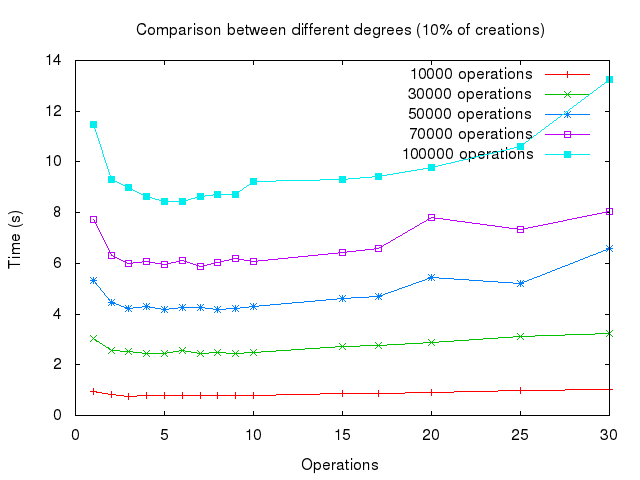
\includegraphics[width=0.95\textwidth]{./plots/cmpLOT10.png}
  \caption{Comparison between B-trees (10\% of insertions)}
  \label{cmpLOT10}
\end{figure}

Figure \ref{cmpLOT30} are the plots for 30\% opertaions being creating an account.
\begin{figure}[htbp]
  \centering
  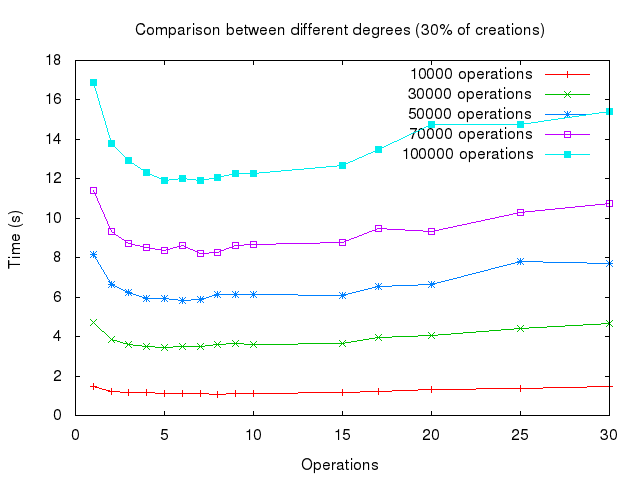
\includegraphics[width=0.95\textwidth]{./plots/cmpLOT30.png}
  \caption{Comparison between B-trees (30\% of insertions)}
  \label{cmpLOT30}
\end{figure}

Figure \ref{cmpLOT70} are the plots for 70\% opertaions being creating an account.
\begin{figure}[htbp]
  \centering
  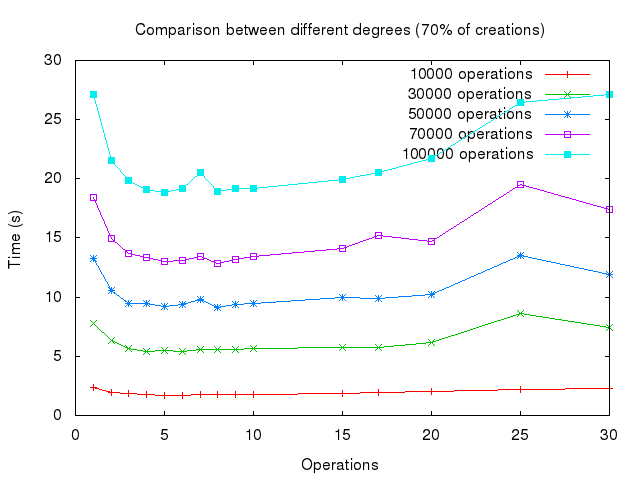
\includegraphics[width=0.95\textwidth]{./plots/cmpLOT70.png}
  \caption{Comparison between B-trees (70\% of insertions)}
  \label{cmpLOT70}
\end{figure}

From above figures, we can conclude that the most suitable degree in current environment is 5 and when it is less or greater it will be less efficient.

\newpage
\appendix
\section{Tools}
During this project, I used these tools: \LaTeXe{}, gnuplot, GitHub.

You can find some plotting scripts for gnuplot in the folder `documentation/plots'. And the respority on GitHub is https://github.com/plusun/Social-Network.git.


\end{document}